%%%%%%%%%%%%%%%%%%%%%%%%%%%%%%%%%%%%%%%%%%%%%%%%%%%%%%%%%%%%%%%%%%%%%%%%%%%%%%%%
%2345678901234567890123456789012345678901234567890123456789012345678901234567890
%        1         2         3         4         5         6         7         8

\documentclass[letterpaper, 10 pt, conference]{ieeeconf}  % Comment this line out if you need a4paper

%\documentclass[a4paper, 10pt, conference]{ieeeconf}      % Use this line for a4 paper

\IEEEoverridecommandlockouts                              % This command is only needed if 
                                                          % you want to use the \thanks command

\overrideIEEEmargins                                      % Needed to meet printer requirements.

% See the \addtolength command later in the file to balance the column lengths
% on the last page of the document

% The following packages can be found on http:\\www.ctan.org
%\usepackage{graphics} % for pdf, bitmapped graphics files
%\usepackage{epsfig} % for postscript graphics files
%\usepackage{mathptmx} % assumes new font selection scheme installed
%\usepackage{times} % assumes new font selection scheme installed
\usepackage{amsmath} % assumes amsmath package installed
\usepackage{bm}
\usepackage{amssymb}  % assumes amsmath package installed
\usepackage{url}
\usepackage{tikz}
\usepackage{tikz-3dplot}
\tdplotsetmaincoords{60}{110}
\usetikzlibrary{fit,shapes,arrows,automata,3d,calc,shapes.geometric}
\usepackage[titlenumbered,longend,ruled,linesnumbered]{algorithm2e}
\usepackage{hyperref}

% random helper commands
\DeclareMathOperator*{\argmin}{argmin}
\DeclareMathOperator*{\argmax}{argmax}
\DeclareMathOperator*{\proj}{proj}
\DeclareMathSymbol{\widehatsym}{\mathord}{largesymbols}{"62}
\newcommand\lowerwidehatsym{%
  \text{\smash{\raisebox{-1.3ex}{%
    $\widehatsym$}}}}
\newcommand\bowler[1]{%
  \mathchoice
    {\accentset{\displaystyle\lowerwidehatsym}{#1}}
    {\accentset{\textstyle\lowerwidehatsym}{#1}}
    {\accentset{\scriptstyle\lowerwidehatsym}{#1}}
    {\accentset{\scriptscriptstyle\lowerwidehatsym}{#1}}
}
\newcommand\mat[2]{\ensuremath{\left[\begin{array}{#1}#2\end{array}\right]}}
\newcommand\deriv[2]{\ensuremath{\frac{\partial #1}{\partial #2}}}
\newcommand{\overbar}[1]{\mkern 4mu\overline{\mkern-4mu#1\mkern-4mu}\mkern 4mu}

% notation
\def\change{ {\mathsmaller\Delta} }
\def\xmat{\uppercase}    \def\xmatstr{in uppercase}
\def\xvec{\vec}          \def\xvecstr{with an arrow}
\def\xuv{\hat}           \def\xuvstr{with a caret}
\def\xse{\bm}            \def\xsestr{in boldface}




\title{\LARGE \bf
Discovery and Estimation of Screw Joint Chains for
Automated Kinematic Modeling
}


\author{Alex Burka and Daniel D. Lee\\
  {\tt \{aburka,ddlee\}@seas.upenn.edu}\\
  Department of Electrical and Systems Engineering\\
  GRASP Laboratory\\
  University of Pennsylvania
}

% this is from http://tex.stackexchange.com/questions/42812/3d-bodies-in-tikz
% I tried to make the parameters configurable and failed
% solution: put this tikzpicture in a node!
% good enough for government work
\newcommand{\tikzhelix}{
  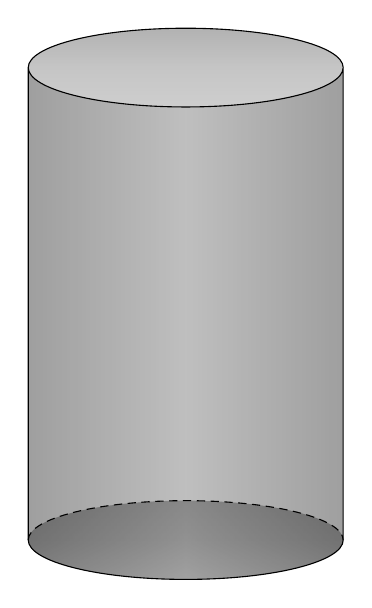
\begin{tikzpicture}[auto]
    \fill[top color=gray!50!black,bottom color=gray!10,middle color=gray,shading=axis,opacity=0.25] (0,0) circle (2cm and 0.5cm);
    \fill[left color=gray!50!black,right color=gray!50!black,middle color=gray!50,shading=axis,opacity=0.25] (2,0) -- (2,6) arc (360:180:2cm and 0.5cm) -- (-2,0) arc (180:360:2cm and 0.5cm);
    \fill[top color=gray!90!,bottom color=gray!2,middle color=gray!30,shading=axis,opacity=0.25] (0,6) circle (2cm and 0.5cm);
    \draw (-2,6) -- (-2,0) arc (180:360:2cm and 0.5cm) -- (2,6) ++ (-2,0) circle (2cm and 0.5cm);
    \draw[densely dashed] (-2,0) arc (180:0:2cm and 0.5cm);
  \end{tikzpicture}
}

\newcommand{\tikzhelixtwo}{
\begin{tikzpicture}[tdplot_main_coords]
  % --- Independent parameters ---
\def\h{3}                          % cylinder height
\pgfmathtruncatemacro\tA{350}      % A angle
\def\zA{0}                         % A applicate
\pgfmathtruncatemacro\tB{120}      % B angle
\def\zB{3}                         % B applicate
\pgfmathtruncatemacro\n{3}         % number of additional turns
\pgfmathtruncatemacro\NbPt{400}     % number of dots for drawing the helix portion
\def\rhelixdots{0.02}              % radius of dots forming helix
\def\rAB{0.05}                     % radius of A and B dots

% --- Draw cylinder ---

% --- Draw helix ---
\pgfmathsetmacro\tone{\tA}
\pgfmathsetmacro\tlast{\tB+\n*360}
\pgfmathsetmacro\ttwo{\tone+(\tlast-\tone)/(\NbPt-1)}
\pgfmathsetmacro\p{360*(\zB-\zA)/(\tB-\tA+360*\n)}
\foreach \t in {\tone,\ttwo,...,\tlast}{%
    \fill[red] ({cos(\t)},{sin(\t)},{\p*(\t-\tA)/360+\zA}) circle[radius=\rhelixdots];
}

% lower circle
\draw[black,very thin] (1,0,0) 
    \foreach \t in {2,3,...,360}
    {
        --({cos(\t)},{sin(\t)},0)
    }
    --cycle;

% upper circle
\draw[black,very thin] (1,0,\h) 
    \foreach \t in {2,4,...,360}
    {
        --({cos(\t)},{sin(\t)},\h)
    }
    --cycle;

% peripheral spokes
    \draw[gray] ({cos(110)},{sin(110)},0)
        --({cos(110)},{sin(110)},\h);
    \draw[gray] ({cos(290)},{sin(290)},0)
        --({cos(290)},{sin(290)},\h);



% labels and lines around the cylinder
\fill (0,0,0) circle[radius=0.1];
\node (center) at (0,.3,0) {$\xvec{o}$};
\draw (0,0,0) -- (0,0,1);
\draw (0,0,1) -- (0,0.1,0.9);
\draw (0,0,1) -- (0,-0.1,0.9);
\node (axis) at (0,0.3,1) {$\xvec{a}$};
\draw (0,0,0) -- (0,-1,0);
\node (radius) at (0.3,-0.5,0) {$r$};
\fill[green] (0,1,2) circle[radius=0.1];
\node (x) at (0,1.3,2) {$\xvec{x}$};
 
\end{tikzpicture}
}

\begin{document}



\maketitle
\thispagestyle{empty}
\pagestyle{empty}


%%%%%%%%%%%%%%%%%%%%%%%%%%%%%%%%%%%%%%%%%%%%%%%%%%%%%%%%%%%%%%%%%%%%%%%%%%%%%%%%
\begin{abstract}
  A difficult problem in perception and manipulation is an automated
  method for discovering and estimating the constrained motions of
  articulated objects.  How can the latent kinematic structure of
  unknown objects be modeled by observing and segmenting the motions
  of their parts in cluttered scenes?  Previous work has used a
  variety of potential joint models to describe the most likely
  kinematic tree from 3-D trajectory data.  In this work, we focus on
  showing how chains of screw joints, which seemlessly integrate
  aspects of both revolute and prismatic joints, can be automatically
  discovered and estimated.  We present an algorithm that
  probabilistically incorporates appropriate noise models on chains of
  screw joints, and show its application in both physical simulation and on
  visual observation of real-world objects.
\end{abstract}


%%%%%%%%%%%%%%%%%%%%%%%%%%%%%%%%%%%%%%%%%%%%%%%%%%%%%%%%%%%%%%%%%%%%%%%%%%%%%%%%

\section{Introduction}

\subsection{Motivation}
As robots become increasingly dexterous and equipped to interact with humans in human environments, there is a pressing need to teach them to use human artifacts (tools, buildings, furniture, vehicles) in a natural and semantically appropriate way. Our work in this area focuses on understanding the kinematic structure of articulated objects (i.e. moving parts) in the environment. Humans rely heavily on intuition, pattern matching and experimentation for this task. For example, sitting down in a rental car may be momentarily disorienting, but a human driver already knows how to operate the pedals, gearshift and windshield wipers. Door locks and radio controls are always different but can be found by analogy, or experimentation if necessary.

By most estimations, the hardware has arrived, but with current software, robots are not very good at intuition, pattern matching and experimentation. Hardcoding separate techniques for interacting with doors, cars, power tools and other objects found in the world, in all their different incarnations of size, shape and appearance gets tiresome very quickly, and is a completely unworkable approach when considering novel objects (such as a new tool, or a broken door). One characteristic of similar objects that tends to remain constant even in the face of cosmetic changes is the underlying kinematic structure; that is, the linkages between different moving parts. The location and types of these linkages define the motion primitives available for an object. For example, a pair of scissors could be broadly defined as two long, thin bars of the same length, connected by a revolute joint in the middle, and free to rotate $180^\circ$. (The handle topology and sharpness of some of the edges are out of the scope of this paper, but see Section \ref{sec:future}.) This description could be used by a sufficiently smart visual system to identify a novel object as scissors, or similar to scissors (e.g. wire cutters, pruning shears, etc). It is therefore more useful than other types of stored patterns, such as a visual template. 
Furthermore, the kinematic model can be extended with dynamic attributes, such as the typical weight of a pair of scissors, and the friction at the revolute joint (see Section \ref{sec:future}).

In the current paper we aim to present a general approach for finding patterns in the motion of objects in a robot's environment. These patterns are discoverable by experimentation, and provide a natural representation of objects which, being directly grounded in the robot's own perceptual and manipulative capabilities, is usable for other tasks such as planning.

\subsection{Literature Review}
%\cite{Sturm2009}, \cite{Aqvist1986}, \cite{Burka2013}

Interactive perception, and discovery of latent kinematic structure, has been investigated previously. It has become somewhat more tractable recently with the widespread availability of accurate RGBD cameras (though in this work, we use a standard RGB camera and recover depth information by instrumenting the environment). Recent work includes the efforts of Dov Katz et al at UMass-Amherst \cite{Katz2008,Katz2008a} and later at CMU \cite{Katz2012}, as well as Yan and Pollefeys at UNC \cite{Yan2006} and J\"{u}rgen Sturm et al at the University of Freiburg \cite{Sturm2011}.

Katz et al present a system for ``interactive segmentation'' as well as kinematic modeling in \cite{Katz2008}. They use three-dimensional (RGBD) vision to track a large cloud of feature points on an articulated object of interest. Then, various metrics are used to group feature points into object parts, including 3D proximity, color and texture consistency, and relative 3D motion (that is, rigidly connected feature points will be close together, possibly the same color, and should have very little relative motion). Once the object of interest is segmented into rigid bodies, they aim to discover the underlying kinematic structure of those bodies. This is done using heuristics specific to each built-in joint type. Specifically, the relative 3D trajectories of feature points on a pair of prismatically connected rigid bodies should fit straight lines, and likewise arcs of circles for a revolute joint. These heuristics are somewhat limiting in that there is no unified system for deriving a heuristic from a kinematic definition. However, in a subsequent paper Katz et al explore the use of reinforcement learning to choose manipulator actions that probe the environment for the sole purpose of perception -- an interesting direction that should be considered for this work as well \cite{Katz2008a}.

Yan and Pollefeys take a more mathematical approach, attempting to discover the motion subspace described by each feature trajectory and linking them by looking for dependencies between the subspaces \cite{Yan2006}. That work is principally applied to non-rigid objects, which puts it outside the scope of this paper, but the approach of considering relative motion as a subspace and representing the object as a graph is relevant.

Sturm et al provide a complete kinematic capture pathway in \cite{Sturm2011}. They seek to create a top-to-bottom system that can go from visual input to a kinematic tree, taking into account mathematical joint models and remaining robust to outliers. Joint types considered are rigid, prismatic, revolute and a catch-all Gaussian process model that can capture several hard-to-model joints, such as a garage door.

\subsection{Screws and Twists}
The literature reviewed above tends to treat joints as modeled by one of several possible models, i.e. a rigid joint or a prismatic joint or a revolute joint. However, these three joint types, as well as combinations thereof, can be unified under the screw joint model. This is consistent with the tradition and terminology of kinematics in general, where a generic three-dimensional rigid motion is represented by a matrix \[ \mat{c|c}{R_{3 \times 3} & t_{3 \times 1} \\\hline 0 & 1} \] This is often called a \emph{screw motion} and it can represent any single rigid motion as a rotation about some axis followed by a translation along the same axis \cite{Murray1994}.

Similarly, in our formalism, as elaborated below, each joint will be represented with a single rotation/translation axis, a radius of rotation, and a pitch describing the ratio between rotation and translation. This allows us to represent prismatic joints, revolute joints, and joints which both translate and rotate (such as a telephoto lens) in a unified, 8-parameter, 1-DOF representation.

For an example, see Figure \ref{fig:tikzoverload}. This shows a schematic screw joint with origin at $\xvec{o}$, axis pointing in the $\xvec{a}$ direction, radius $r$ and some arbitrary pitch $p$ (not pictured). The cylinder and helix illustrate the possible range of motion. A position of the joint, with the degree of freedom set to a variable $\theta$, may be calculated from
\begin{align}
  \xvec{x} &= \textsc{R}(\xvec{a},\theta,r) \cdot \textsc{T}(\xvec{a},\theta p) \cdot \xvec{o} \label{eq:forward}
\end{align}
  where
  $\textsc{R}(\xvec{n},\theta,r)$ is a rotation about axis $\xvec{n}$ by an angle $\theta$, with radius $r$
  and
  $\textsc{T}(\xvec{n},d)$ is a translation along axis $\xvec{n}$ by distance $d$.

\begin{figure}[ht]
  \centering
  \begin{tikzpicture}[auto]
    \node (test) [scale=1.5,rotate=20] at (0,0) {\tikzhelixtwo{}};
  \end{tikzpicture}
  \caption{Schematic screw joint}
  \label{fig:tikzoverload}
\end{figure}
\section{Articulated Objects as Screw Joint Trees}
Many everyday objects have several moving parts. The joints which connect two moving parts may be characterized by joint type and number of degrees of freedom (DoG). In this paper we will consider only joints with one degree of freedom. This covers most objects, though to represent some joints we would need two (such as a swivel chair which both rotates and extends) or even three (in the case of a ball-and-socket joint).

Furthermore, the only considered joint type will be the screw joint. Conceptually, a screw joint links two object parts $a$ and $b$ with one degree of freedom such that $b$ translates and rotates along the same axis with respect to $a$. The ratio between rotation and translation is the \emph{pitch}. Considering only this joint type is not so limiting as it seems, because the common joint types (i.e. those covered in \cite{Sturm2011}) exist as degenerate cases. A prismatic joint is simply a screw joint with infinite pitch, whereas a revolute joint is a screw joint with zero pitch.

In general, an object with many moving parts must be modeled by a connected, directed graph where the vertices are object parts and the edges are joints.  Any node of indegree greater than unity has extra implied kinematic constraints. In this work these will be ignored, so all graphs in question will be trees. For an example, consider the two-axis translation table depicted in Figure \ref{fig:example} with its associated kinematic tree model. The long bars translate in two dimensions, and the red knobs control each axis. This tree contains both screw joints (the X knob with respect to the base, and the Y knob with respect to the X gantry) and prismatic joints, or infinite-pitch screw joints (the sliding gantries). Note that this is not the only possible model: the knobs could be modeled as connected to their respective gantries, where they would be pure revolute joints, or zero-pitch screws. Also, this model ignores the fact that the rotary motion of the knobs is causally related to the translation of the gantries: it is a kinematic model, not a dynamic one.

\begin{figure}[ht]
  \centering
  \begin{tikzpicture}[auto]
    \tikzstyle{node} = [draw, ellipse, font=\small, align=center]

    \node (base) at (5.5,0.75) [node, accepting] {base};
    \node (xslide) [node, below of=base, node distance=4em, text width=2em] {X gantry};
    \node (yslide) [node, below of=xslide, node distance=5em, text width=2em] {Y gantry};
    \node (xknob) [node, left of=xslide, node distance=6em, text width=1.5em] {X knob};
    \node (yknob) [node, left of=yslide, node distance=6em, text width=1.5em] {Y knob};

    \draw [->] (base) -- node {Pr} (xslide);
    \draw [->] (xslide) -- node {Pr} (yslide);
    \draw [->] (base) -- node[above] {Sc} (xknob);
    \draw [->] (xslide) -- node[above] {Sc} (yknob);

    \node (image) {\includegraphics[width=0.25\textwidth]{img/axistable.jpg}};
    \node (knx) at (-1.35,-0.05) {};
    \node (kny) at (1,-0.25) {};
    \draw [-,dashed,ultra thick,green] (xknob.north) to[bend right] node {} (knx);
    \draw [-,dashed,ultra thick,green] (yknob.west) to[bend left] node {} (kny);

    \node (xg1) at (-0.5,-0.1) {};
    \node (xg2) at (-1.1,-0.6) {};
    \node (yg1) at (-0.85,0.75) {};
    \node (yg2) at (-1.5,1.05) {};
    \draw [<->,line width=2pt,blue] (xg1) -- node {} (xg2);
    \draw [<->,line width=2pt,blue] (yg1) -- node {} (yg2);
  \end{tikzpicture}
  \caption{Two axis table}
  \label{fig:example}
\end{figure}

\section{Model Fitting}
Input to the model comes in the form of 6D trajectories, which will be denoted by the rigid transform matrix representation, i.e. $\xse{x} = \mat{ccc|c}{&&& t_x \\ & \xmat{r} && t_y \\ &&& t_z \\\hline 0 & 0 & 0 & 1}$.\footnote{In this paper, superscripts are used for numbering object parts, feature points or graph/tree edges, while subscripts are reserved for indexing in time. Where it makes sense, operations may be considered to be implicitly vectorized (i.e. $(\xse{x}_{1..T}^a)^{-1}$ refers to $\{(\xse{x}_1^a)^{-1}, (\xse{x}_2^a)^{-1}), \dots\}$). Also, elements of $SE(3)$ will usually be shown \xsestr{} ($\xse{x}$), matrices in $\mathbb{R}^{3 \times 3}$ \xmatstr{} ($\xmat{a}$), vectors in $\mathbb{R}^2$ or $\mathbb{R}^3$ \xvecstr{} ($\xvec{v}$), and unit vectors in $\mathbb{U}^2$ or $\mathbb{U}^3$ \xuvstr{ } ($\xuv{u}$).} The full trajectory describing an object with $K$ parts over $T$ timesteps is
\begin{align}
  X = \{ \xse{x}_t^k \in SE(3) \mid k \in \{1..K\}, t \in \{1..T\} \}
\end{align}
To fit the individual joint models, the relative transformations are more useful, so for every pair of objects $a, b \in 1..K$ we will refer to the \emph{deltas}:
\begin{align}
  \xse{\Delta}_{1..T}^{a:b} &= \xse{x}_{1..T}^{b} (\xse{x}_{1..T}^{a})^{-1}
\end{align}
Using these deltas, we can treat each joint independently as if only one part is moving and the other is stationary at the origin.

\begin{figure}[ht]
  \centering
  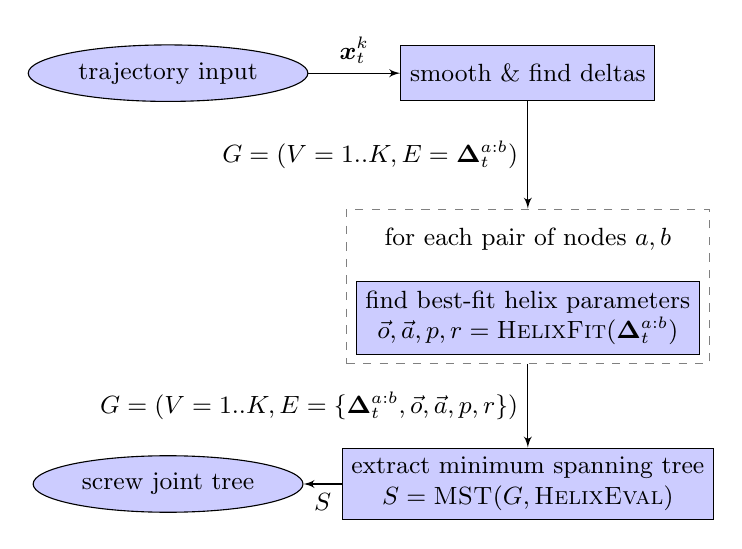
\begin{tikzpicture}[auto, >=latex']
    \tikzstyle{every node} = [font=\small]
    \tikzstyle{textbox} = [align=center, draw, fill=blue!20, minimum height=2em, minimum width=4em]
    \tikzstyle{block} = [textbox, ellipse]
    \tikzstyle{function} = [textbox, rectangle]
    \tikzstyle{pinstyle} = [pin edge={to-,thin,black}]

    \node (input) [block] {trajectory input};
    \node (preprocess) [function, right of=input, node distance=13em] {smooth \& find deltas};
    \node (loop) [below of=preprocess, node distance=6em] {for each pair of nodes $a, b$};
    \node (fit) [function, below of=loop] {find best-fit helix parameters \\ $\xvec{o}, \xvec{a}, p,r = \textsc{HelixFit}(\xse{\Delta}_t^{a:b})$};
    \node (mst) [function, below of=fit, node distance=6em] {extract minimum spanning tree \\ $S = \textsc{MST}(G, \textsc{HelixEval})$};
    \node (output) [block, left of=mst, node distance=13em] {screw joint tree};

    \node (box) [draw=black!50, dashed, fit={(loop) (fit)}] {};
    \draw [->] (input) -- node {$\xse{x}_t^k$} (preprocess);
    \draw [->] (preprocess) -- node[left] {$G=(V=1..K, E=\xse{\Delta}_t^{a:b})$} (box);
    \draw [->] (box) -- node[left] {$G=(V=1..K, E=\{\xse{\Delta}_t^{a:b}, \xvec{o},\xvec{a},p,r\})$} (mst);
    \draw [->] (mst) -- node {$S$} (output);
  \end{tikzpicture}
  \caption{Block diagram of model fitting process}
  \label{fig:block-algo}
\end{figure}

A helix requires 8 parameters for a complete specification: the origin $\xvec{o} \in \mathbb{R}^3$, the axis $\xuv{a} \in \mathbb{U}^3$, the radius $r \in \mathbb{R}$ and pitch $p \in \mathbb{R}$. The quadratic constraint that the axis must be a unit vector means that this is a 7-dimensional configuration space.

This algorithm uses only the translation components of the 6D trajectories, reducing the dimension of the input space to 3 but possibly discarding useful data (see Section \ref{sec:future}). We assume that the input points are independent and identically distributed, sampled from a distribution centered at the helix trajectory (i.e. (\ref{eq:forward}) with Gaussian noise). The goal is to find the maximum likelihood solution, that is, the parameters $\xvec{o}$, $\xvec{a}$, $r$ and $p$ which maximize the probability of generating data similar to the input. Since the noise model is Gaussian, we use ordinary least squares fitting. Another possible noise model is Laplacian, where iteratively reweighted least squares (IRLS) would be appropriate to simulate a linear objective, but this was not observed to affect the fitting results.

The fitting proceeds in three steps, detailed in Alg. \ref{alg:fit}.

The first step, which is the harder and more important of the two, is to find the helix origin and axis. Our approach is to treat the trajectory as a point cloud in 3D space, and perform a principal components analysis (PCA) to find the dominant directions present in the cloud. One of the principal axes will be used as an initial estimate of the helix axis. (If the helix is long and narrow, it will be the component that describes the most variation, but we cannot assume this since the helix could be shallow, or it may not even contain a complete revolution.) We choose for the estimate the component which collapses the helix into the ``best'' circle. ``Best'' here is determined by projecting the helix down onto a plane (line \ref{alg:fit:proj}), fitting a circle (Algorithm \ref{alg:fit-findcenter}) and checking the deviation from the fitted radius (line \ref{alg:fit:ei}).

The second step, given the axis, finds the helix radius and pitch. The joint state ($\theta$) at each timestep is produced as a byproduct of this step. Our approach is to take the projected helix (produced in the first step), where it should form an arc of a circle. Then we can extract the rotation angle at each timestep (line \ref{alg:fit:atan}). This provides an estimate of the radius, and a simple linear regression (line \ref{alg:fit:linreg}) from rotation angle to height above the plane gives the pitch.

Lastly, we refine the estimates of the helix origin and axis by means of nonlinear optimization (in this implemention, using the COBYLA algorithm \cite{cobyla} as implemented by NLopt \cite{nlopt}), contraining the axis to be a unit vector, and using as the objective function the circularity of the helix plane projection. Then the calculations of step 2 are repeated, given the refined estimates.

\begin{algorithm}[h]
  \SetFuncSty{textsc}
  \SetProcNameSty{textsc}
  \caption{Helix Fitting Procedure}
  \label{alg:fit}
  \KwIn{$\xvec{y}_{1..T}$ relative trajectory of point $b$ (point $a$ stays at the origin)}
  \KwOut{Helix parameters $\{\xvec{o}, \xvec{a}, p, r\}$}
  \SetKwFunction{PCA}{PCA}
  \SetKwFunction{Plane}{Plane}
  \SetKwFunction{Project}{Proj}
  \SetKwFunction{LinReg}{LinReg}
  \SetKwFunction{FindCenter}{FindCenter}
  \SetKwFunction{Circularity}{Circularity}
  \SetKwFunction{Optimize}{Opt}
  \SetKw{KwInn}{in}
  \DontPrintSemicolon
  \BlankLine

  \tcp{Step 1: find helix origin/axis}
    $\xvec{b}^{1..3}, \xvec{z}_{1..T} \leftarrow \PCA(\xvec{y}_{1..T})$ \;
    \For{$i$ \KwInn $\{1..3\}$}{
      $c \leftarrow \frac{1}{T}\sum_t \xvec{z}_t$ \;
      $c[i] \leftarrow \min_t \xvec{z}_t(i)$ \;
      $plane \leftarrow \Plane(c, b^i)$ \;
      $\xvec{u}_{1..T}^i \leftarrow \Project(plane, \xvec{y}_{1..T})$ \label{alg:fit:proj} \;
      $\xvec{o}^i, r^i \leftarrow \FindCenter(\xvec{u}_{1..T})$ \;
      $e^i \leftarrow \sum_t ( ||\xvec{u}_t - \xvec{o}^i|| )^2$ \label{alg:fit:ei} \;
    }
    $h \leftarrow \argmin_i e^i$ \;
    $\xvec{u}_{1..T}, \hat{\xvec{o}}, \hat{\xvec{a}}, \hat{r} \leftarrow \xvec{u}_{1..T}^h, \xvec{o}^h, \xvec{a}^h, r^h$ \;
  \tcp{Step 2: extract angles and pitch}
    $\theta_{1..T} \leftarrow \tan^{-1}(\frac{\xvec{u}_{1..T}[2] - \hat{\xvec{o}}[2]}{\xvec{u}_{1..T}[1] - \hat{\xvec{o}}[1]})$ \label{alg:fit:atan} \;
    $\hat{p} \leftarrow \LinReg(\theta_{1..T}, \xvec{y}_{1..T} \cdot \hat{\xvec{a}})$ \label{alg:fit:linreg} \;

  \tcp{Step 3: nonlinear optimization}
    $\hat{\xvec{o}}, \hat{\xvec{a}} \leftarrow \Optimize(\Circularity(\xvec{y}_{1..T}, \xvec{o}, \xvec{a}), ||\xvec{a}||=1, \hat{\xvec{o}}, \hat{\xvec{a}})$ \;
    $plane \leftarrow \Plane(\hat{\xvec{o}}, \hat{\xvec{a}})$ \;
    $\xvec{u}_{1..T}^i \leftarrow \Project(plane, \xvec{y}_{1..T})$ \;
    $\theta_{1..T} \leftarrow \tan^{-1}(\frac{\xvec{u}_{1..T}[2] - \hat{\xvec{o}}[2]}{\xvec{u}_{1..T}[1] - \hat{\xvec{o}}[1]})$ \;
    $\hat{p} \leftarrow \LinReg(\theta_{1..T}, \xvec{y}_{1..T} \cdot \hat{\xvec{a}})$ \;
\end{algorithm}

\begin{algorithm}[h]
  \SetFuncSty{textsc}
  \SetProcNameSty{textsc}
  \caption{\textsc{FindCenter} (subroutine for Alg. \ref{alg:fit})}
  \label{alg:fit-findcenter}
  \KwIn{$\xvec{u}_{1..T}$ set of coplanar 2D points}
  \KwOut{$\xvec{o}$ center, $r$ radius}
  \DontPrintSemicolon
  \BlankLine

  $\xvec{a} \leftarrow \mat{cc}{\xvec{u}_{1..T} & \xvec{1}_{T \times 1}}_{T \times 3}^{-1} * \mat{c}{-||\xvec{u}_{1..T}||^2}_{T \times 1}$ \;
  $\xvec{o} \leftarrow \mat{cc}{\xvec{a}[1] & \xvec{a}[2]}$ \;
  $r \leftarrow \xvec{a}[3]$ \;

\end{algorithm}

\begin{algorithm}[h]
  \SetFuncSty{textsc}
  \SetProcNameSty{textsc}
  \caption{\textsc{Circularity} (subroutine for Alg. \ref{alg:fit})}
  \label{alg:fit-circularity}
  \KwIn{$\xvec{y}_{1..T}$ set of 3D points, $\xvec{o}$ plane origin, $\xvec{a}$ plane normal}
  \KwOut{$e$ circularity score}
  \SetKwFunction{Plane}{Plane}
  \SetKwFunction{Project}{Proj}
  \SetKwFunction{FindCenter}{FindCenter}
  \SetKwFunction{Std}{Std}
  \DontPrintSemicolon
  \BlankLine

  $plane \leftarrow \Plane(\xvec{o}, \xvec{a})$ \;
  $\xvec{u}_{1..T} \leftarrow \Project(plane, \xvec{y}_{1..T})$ \;
  $\xvec{o} \leftarrow \FindCenter(\xvec{u}_{1..T})$ \;
  $e \leftarrow \Std( \sum_t || \xvec{u}_t - \xvec{o} || )$ \;

\end{algorithm}

Finally, the best circularity value returned by the optimization function is used as the ``score'' of the proposed joint. Since we evaluate every pairing of objects parts as a potential screw joint, but seek a tree as the final model, the minimum spanning tree is selected (by Prim's algorithm \cite{prim}), using the joint scores as edge weights.

\section{Evaluation}
The helix fitting system has been evaluted both in simulation and using real-world data captured from the robotic arm pictured in Figure \ref{fig:arm}.

\subsection{Simulation}

The goal of the simulation experiment is to define a screw joint by its parameters, and generate a trajectory by executing a random walk in state space. At this point noise is added, and we hope to recover the original helix parameters from the noisy trajectory by Algorithm \ref{alg:fit}.

The forward kinematics of a screw joint, as applied to a vector $\xvec{v}$, are given by the following chain of rigid transformations, read from right to left. First, $\xse{c}$ moves the origin to the helix origin and aligns the $z$-axis with the helix axis. \textsc{T} and \textsc{R} generate pure translation and rotation about the $z$-axis. Then $\xse{r}$ incorporates the helix radius.
\begin{align}
  \xse{s} \cdot \xvec{v} &= \xse{r} \cdot \textsc{R}(0, 0, \theta) \cdot \textsc{T}(0, 0, \theta p) \cdot \xse{c} \cdot \xvec{v}
\end{align}
(More specifically, we use the parametrized rigid transforms $\textsc{R}(\theta_1, \theta_2, \theta_3)$, a rotation given $ZYZ$ Euler angles and $\textsc{T}(d_x, d_y, d_z)$, an axis-aligned translation.) With two rigid transformations, plus the pitch, totaling 13 parameters, this representation is richer than the 7-dimensional description of a helix given earlier. This is due to the fact that $\xse{r}$ can incorporate an arbitrary post-transformation as long as it maintains a constant helix radius, and $\xse{c}$ must align the $z$-axis but may rotate the $xy$-plane. This accounts for the extra 6 parameters. Though the full parametrization is necessary for modeling general kinematic chains without resorting to intermediate rigid joints, here for the purposes of simulation we will restrict $\xse{c}$ to a simple translation and rotation, and $\xse{r}$ to a one-dimensional translation.

The simulator is controlled by a graphical interface, shown in Figure \ref{fig:gui}. It contains a tree editor and can simulate arbitrary kinematic chains of rigid, prismatic, revolute and screw joints (the last was added for this work). The source code and data files used to generate the simulated trajectories used here can be found in Appendix \ref{sec:code}.

\begin{figure}[ht]
  \centering
  \includegraphics[width=.47\textwidth]{img/screenshot.png}
  \caption{Custom GUI for designing and simulating articulated objects}
  \label{fig:gui}
\end{figure}

For this experiment, two screw joints were simulated. Both have an origin at $(0, 0, 0)$, a helix axis of $(0, 0, 1)$ and a radius of 1. One joint has a pitch of 0 (making it a revolute joint) and the other has a pitch of 5. Table \ref{tbl:simulation} shows the learned parameters.

\begin{table}[ht]
  \begin{tabular}{c|c|c|c|c}
           & \multicolumn{2}{c}{Revolute} & \multicolumn{2}{|c}{Screw} \\
           & Simulated   & Detected    & Simulated   & Detected    \\ \hline
           Origin & $\mat{c}{0 \\ 0 \\ 0}$ & $\mat{c}{0.0005 \\ -0.0065 \\ 0.0008}$ & $\mat{c}{0 \\ 0 \\ 0}$ & $\mat{c}{0.2682 \\ 0.2546 \\ -0.0011}$ \\
    Axis   & $\mat{c}{0 \\ 0 \\ 1}$ & $\mat{c}{-0.0654 \\ 0.1154 \\ 0.9912}$ & $\mat{c}{0 \\ 0 \\ 1}$ & $\mat{c}{0.0035 \\ 0.0006 \\ 1.000}$ \\
    Radius & 1           & 1.5583      & 1           & 1.0980      \\
    Pitch  & 0           & 0.0175      & 5           & 4.9240      \\
  \end{tabular}
  \caption{Parameters through the simulation}
  \label{tbl:simulation}
\end{table}

The simulated parameters were detected relatively well. In particular, the crucial difference between the two joints, namely the pitch, comes through quite accurately.

\subsection{Robotic Arm}
The main experiment focused on a robotic arm made out of Dynamixel servomotors (pictured at left in Figure \ref{fig:arm}) as the articulated object of interest. In particular, there are four revolute joints (base, shoulder, elbow and wrist) as well as a prismatic joint that was not used in this experiment. This makes the arm a versatile object in the context of our system which models 1-DOF joints.

\begin{figure}[ht]
  \centering
  \includegraphics[width=0.3\textwidth]{img/arm.png}
  \caption{Robotic arm instrumented with Aruco tags}
  \label{fig:arm}
\end{figure}

In the figure the labeled joints are indicated, with markers on the shoulder, upper arm, lower arm, and wrist. In this experiment, we exclude the shoulder marker because the camera capture system has low resolution in the out-of-page direction, so from this angle it is difficult to observe the shoulder joint. (But see Section \ref{sec:future}.) Detection is performed on the revolute elbow and wrist joints, both of which rotate in planes roughly parallel to the image plane.

Images were captured using a Logitech C905 webcam, at a resolution of 1600x1200 (decimated to 800x600 to make near-real-time processing feasible), and processed using a custom-written program on a commodity Macbook Air (links to the code and data are available in Appendix \ref{sec:code}).

Figure \ref{fig:results} shows the robotic arm in an augmented-reality view highlighting the markers and, in red, the axes and ranges of motion of the detected screw joints. In fact, the range-of-motion tracks are helices, but these are both revolute joints, with low pitches, so they appear as nearly planar circles.

\begin{figure}[ht]
  \centering
  \includegraphics[width=0.4\textwidth]{img/omgcircles.png}
  \footnotesize
  \begin{tabular}{c|c|c|c}
    & \multicolumn{1}{c}{Joint 1 (bottom)} & \multicolumn{2}{|c}{Joint 2 (top)} \\
    & Detected    & Truth   & Detected    \\ \hline
    Origin & $\mat{c}{-14.90 \\ 37.65 \\ -3.118}$ & $\mat{c}{-14.90 \\ 55.15 \\ 3.362}$ & $\mat{c}{-16.75 \\ 51.89 \\ 2.520}$ \\
    Axis   & $\mat{c}{-0.077 \\ 0.994 \\ 0.077}$ & $\mat{c}{0 \\ 1 \\ 0}$ & $\mat{c}{0.034 \\ 0.999 \\ 0.038}$ \\
    Radius & 15.7749      & 18.75           & 13.8298      \\
    Pitch  & -0.24913      & 0           & -0.610883      \\
  \end{tabular}
  \caption{Rendered tracks showing range of motion of detected joints}
  \label{fig:results}
\end{figure}

In the table above, the lower joint is used to calibrate the coordinate system, so its origin and radius are taken as true. Measurements of the apparatus were then scaled to create ground truth for the upper joint. Inspection shows that, accounting for inaccuracies in measurement and in tag capture, the detection performance is reasonable.

%seas1366:py alex$ screen /dev/tty.usbserial-A700dBdS 9600
%=== Dynamixel controller initialized ===
%J shoulder 2- 3+
%Created joint shoulder
%J elbow 4- 5+
%Created joint elbow
%r 2 3 4 5
%Motor #2 position = 331, load = 0
%Motor #3 position = 697, load = 0
%Motor #4 position = 448, load = 0
%Motor #5 position = 568, load = 0
%j shoulder 200
%Moving motor #2 to position 131
%Moving motor #3 to position 897
%j shoulder -200
%Moving motor #2 to position 531
%Moving motor #3 to position 497
%j elbow 200
%Moving motor #4 to position 248
%Moving motor #5 to position 768
%j elbow -250
%Moving motor #4 to position 698
%Moving motor #5 to position 318
%j shoulder 200
%Moving motor #2 to position 131
%Moving motor #3 to position 897
%j elbow 200
%Moving motor #4 to position 248
%Moving motor #5 to position 768
%H elbow shoulder
%Moving motor #4 to position 448
%Moving motor #5 to position 568
%Moving motor #2 to position 331
%Moving motor #3 to position 697

%[fitter thread] 		RESULT
%[fitter thread] 			caxis: [0.03437679864999697, 0.9986694754396289, 0.03843845131784304]
%[fitter thread] 			origin: [-16.75012155215985, 51.88951473647936, 2.515950958262303]
%[fitter thread] 			plane: [-16.75012155216786, 51.88951473647964, 2.515950958262278], [0, 0.03846118406286526, -0.9992600949304853], [-0.9994089431832086, 0.03435136308240214, 0.001322172380369591]
%[fitter thread] 			radius: 13.8298
%[fitter thread] 			pitch: -0.610883
%[fitter thread] computing minimum spanning tree...
%[fitter thread] 	before: 0->1 (0.0661745)
%[fitter thread] 	before: 0->2 (2.10676)
%[fitter thread] 	before: 1->2 (0.0846317)
%[fitter thread] 	crunch...
%[fitter thread] 	after: 0->1
%[fitter thread] 	after: 1->2
%[graphics thread] Joint from 0 to 1 with score 0.0661745
%[graphics thread] 	origin=[-14.90110372722932, 37.65122395588835, -3.118204715635848], axis=[-0.07667915242531208, 0.9941174254504841, 0.07649086219305651], radius=15.7749, pitch=-0.24913
%[graphics thread] Joint from 1 to 2 with score 0.0846317
%[graphics thread] 	origin=[-16.75012155215985, 51.88951473647936, 2.515950958262303], axis=[0.03437679864999697, 0.9986694754396289, 0.03843845131784304], radius=13.8298, pitch=-0.610883

\section{Conclusions and Future Work} \label{sec:future}

In this paper we have presented a system for capturing the kinematic structure of an articulated object, as modeled by a tree of screw joints. Screw joints are general enough to capture the common types of 1-DOF joints: prismatic, revolute, and screw. Within our framework the models produced are perceptually grounded and so they are applicable to many other tasks that a robot needs to perform in a human environment. There are also ample avenues for future work. Robustness is always a problem, and a system that will be applicable in diverse applications should be very robust to changes in environment, lighting, etc. Part of the solution to this problem is to revamp the input pathway. The fiducials should be replaced by a more robust visual system, using stereoscopic vision to track features with no need to instrument the environment. Also, the fitting may benefit from considering the full 6D input (including orientation). On the other end of the system, the kinematic model can be made more useful with the addition of information about dynamics, such as the weight of objects and the charatistics of joints (range of motion, friction, etc). With a basic kinematic model in place, the robot can experiment with an object, exercising the discovered degrees of freedom in order to discover new ones and refine the model.

\appendix

\subsection{Source Code} \label{sec:code}
The Kinematic Arboretum simulator is implemented in Matlab. Implementations of the helix fitting algorithm are available both in Matlab and C++ (much faster). The C++ program is also used for gathering camera data and extracting the trajectory data for input to the Matlab fitter. All of the source code is available at \url{http://www.alexburka.com/penn/manip.php}.


\subsection{Acknowledgements}
This work was supported by the National Science Foundation and the Army Research Laboratory.



\bibliographystyle{plain}
\bibliography{IEEEabrv,research}




\end{document}
